% In the batch queue,  queue time becomes dominant but, at the same time, we
% have more freedom to decide the parameters of the slot.

\subsection{Experiments}

In this section we describe experiments that have been performed by running the ATLAS workload on TITAN's batch queue by means of the next generation executor (NGE) \jhanote{We'll need to reference the section/sub-section where this is discussed}.

The importance \jhanote{aim?} of these experiments is twofold: on the one side, we illustrate the performances of the NGE; on the other side, they help to characterize TITAN's batch queue and we show that it can be used as alternative to backfilling. Since we aim to study the response time of batch queue as it is perceived by a common user,  special privileges have been asked to system administrator. \jhanote{I don't think the second point captures accurately why we are interested in the NGE. Please refine}

%This is particularly important for the development of future execution strategies because queue time becomes dominant in

Experiments aim to show \jhanote{calculate? determine?} the number of completed events as function of the time.
Each experiment corresponds to a number of different and independent runs that is meaningful from a statistical point of view. \jhanote{previous sentence needs fixing} Each run consists of a sustained execution of the ATLAS workload for a pre-determined period of time \aanote{A week? 10 days?}. \jhanote{How do we determine this time window?} Since execution of events is carried on by means \jhanote{what is an NGE job?} NGE jobs, each run is based on a script that maintains constant pressure on TITAN's batch queue. \jhanote{please separate what we are trying to achieve from how..}

The main tasks of the script are to:  i) guarantee that there are constantly four NGE jobs eligible for running on TITAN's queue (note that four jobs is the maximum allowed in TITAN's batch queue \ref{}); ii)  bind Athena-MP jobs to the NGE jobs; iii) perform garbage collection. No limit in the number of NGE jobs is imposed.

The simulation of events is due to the following execution model: the script\jhanote{the script is too casual/imprecise} binds a number of Athena-MP jobs that is equal to the number of nodes on which NGE job is running; then, NGE job spawns the Athena-MP jobs on the nodes; finally, the Athena-MP jobs will simulate a number of events that is proportional to the wall-time of the NGE job. As a consequence, the number of nodes determines the number of events that can be simulated concurrently whereas the wall-time determines the number of events that can be simulated one after the other. These two parameters together determine the size of the NGE job. \jhanote{please refine. difficult to understand}

The size of the NGE job is constant within an experiment. Thus, each experiment is fully characterized by the size of the NGE jobs that it send on the nodes.

Each execution of Athena-MP is guaranteed to be successfull and, on average, comparable with those executed by PanDA in production.

Table \ref{tab:experiments} provides the list of the experiments that have been performed.

\begin{table*}
\begin{center}
\begin{tabular}{|c|l|l|l|l|}
  \hline
Experiment &\# nodes &wall-time (hours) & run duration(days) & \# runs   \\
\hline
1 & &  & &   \\
2 & &  & &  \\
3 & &  & &  \\
4 & &  & &  \\
\hline
\end{tabular}
\end{center}
\caption{List of experiments}\label{tab:experiments}
\end{table*}

Each experiment has been designed by choosing the maximum number of nodes and the maximum wall-time of each TITAN bin \ref{} \aanote{Are we really doing this???}. The length of the experiment has been decided.....\aanote{It was 10 times the wall-time or something like that}.

Figure \ref{fig:avtEvts} \aanote{(DRAFT)}depicts average number of completed events as function of the time. Figure \ref{fig:avtTimes} \aanote{(DRAFT)} depicts the average queue time and execution time per experiment.

\begin{figure}[!htb]
        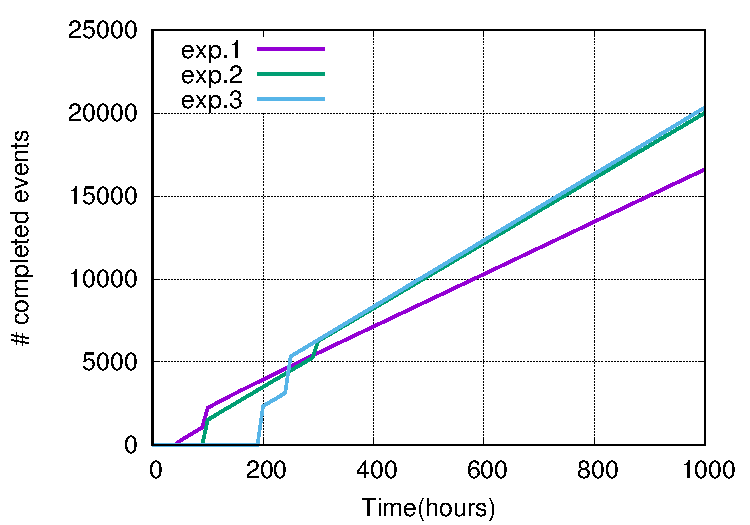
\includegraphics[width=0.48\textwidth]{./figures/draft/mean.pdf}
    \caption{Average number of completed as function of the time.}
\label{fig:avtEvts}
\end{figure}

\begin{figure}[!htb]
        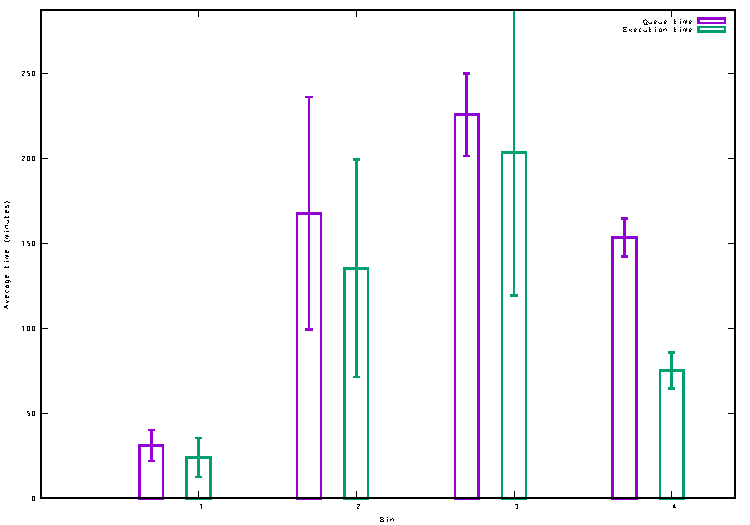
\includegraphics[width=0.48\textwidth]{./figures/draft/AvgT.pdf}
    \caption{Average queue time and execution time of the experiments.}
\label{fig:avtTimes}
\end{figure}

Because of the definition of the experiment the results shown in Figure \ref{} are alike (but not entirely comparable to) those provided by in Figure \ref{} where the performances of backfilling are shown.









% For this reason, the second set of the experiments aims to find
%sub-optimal parameters with which we can minimize the trade-off between the size
%of a slot and the time spent in queue waiting for that slot to become available.
%In other words, we aim to minimize the completion time by finding the best
%trade-off between execution time and queue time.
%
%This execution model introduces slot utilization as one of the key factors for
%high-performances. This happens because, in order to minimize the time spent in
%queue, we might asks for slots in advance and, then we could not be able to
%saturate them when they become available. Thus, this strategy requires a new
%functionality that allows the job to receive and execute new events while it is
%already running on the resources. In order to do that we perform the experiments
%by using a new generation executor that implements such functionality.
%
%As last observation, it is important to point out that the percentage of
%utilization of a slot is minor problem with the current implementation because,
%due to the dynamics of the Backfill queue, PanDA has a high probability to
%re-acquire a slot immediately after it has released one\aanote{Are we able to
%quantify this ``immediately''?}.
